\documentclass[11pt,a4paper]{report}
\usepackage[margin=0.5in]{geometry}
\usepackage[explicit]{titlesec}
\usepackage[dvipsnames]{color}
\usepackage{graphicx}
\usepackage{wrapfig}
\usepackage{lscape}
\usepackage{rotating}
\usepackage{epstopdf}

\definecolor{mygray}{gray}{.75}

\titleformat{name=\section,numberless}[display]
  {\normalfont\scshape\Large}
  {\hspace*{-10pt}#1}
  {-15pt}
  {\hspace*{-110pt}\rule{\dimexpr\textwidth+80pt\relax}{2pt}\Huge}
\titlespacing*{\section}{0pt}{30pt}{10pt}

\titleformat{name=\subsection,numberless}[display]
  {\normalfont\scshape}
  {\hspace*{-10pt}#1}
  {-15pt}
  {\hspace*{-110pt}\rule{\dimexpr\textwidth+30pt\relax}{0.4pt}\Huge}
\titlespacing*{\subsection}{0pt}{20pt}{5pt}


\begin{document}

\noindent\Large\textbf{CM2101 (Human-Computer Interaction)}\\
\noindent\large\textit{Non-assessed Tutorial 2}
\vskip30pt

\section*{Solutions}

\begin{enumerate}

    \item   
        \begin{itemize}
            \item Identify goals and subgoals
                \begin{itemize}
                    \item Goal: Reserve tickets
                    \item Subgoals
                    \begin{itemize}
                        \item Select movie
                        \item Select time
                        \item Choose tickets
                    \end{itemize}
                \end{itemize}
                \item Identify operators
                    \begin{itemize}
                        \item Move mouse to \texttt{<LOCATION>}
                        \item Click mouse
                        \item Depress mouse button
                        \item Release mouse button
                        \item Decide if \texttt{<X>} then \texttt{<Y>}
                    \end{itemize}
                \item Identify methods
                    \begin{itemize}
                        \item Top level goal
                            \begin{enumerate}
                                \item Complete goal: \texttt{RESERVE\_TICKETS}
                            \end{enumerate}
                        \item Method for goal: \texttt{RESERVE\_TICKETS}
                            \begin{enumerate}
                                \item Complete goal: \texttt{SELECT\_MOVIE(movie)}
                                \item Complete goal: \texttt{SELECT\_TIME(time)}
                                \item Complete goal: \texttt{CHOOSE\_TICKETS(num\_tickets)}
                            \end{enumerate}
                        \item Method for goal: \texttt{SELECT\_MOVIE(movie)}
                            \begin{enumerate}
                                \item Move mouse to \textbf{movie selection box}
                                \item Click mouse
                                \item Move mouse to \texttt{movie}
                                \item Click mouse
                                \item Move mouse to \textbf{continue button}
                                \item Click mouse
                                \item Return with goal completed
                            \end{enumerate}
                        \item Method for goal: \texttt{SELECT\_TIME(time)}
                            \begin{enumerate}
                                \item Move mouse to \textbf{button representing \texttt{time}}
                                \item Click mouse
                                \item Return with goal completed
                            \end{enumerate}
                        \item Method for goal: \texttt{CHOOSE\_TICKETS(num\_tickets) 1}
                            \begin{enumerate}
                                \item Move mouse to \textbf{increment ticket count button}
                                \item Click mouse
                                \item Decide if \textbf{displayed count = \texttt{num\_tickets}} then \textbf{return with goal completed}
                                \item Return to step (b)
                            \end{enumerate}
                        \item Method for goal: \texttt{CHOOSE\_TICKETS(num\_tickets) 2}
                            \begin{enumerate}
                                \item Move mouse to \textbf{increment ticket count button}  
                                \item Depress mouse button
                                \item Wait until \textbf{displayed count = \texttt{num\_tickets}}
                                \item Release mouse button
                                \item Return with goal completed
                            \end{enumerate}
                    \end{itemize}
                \item Identify selection rules
                    \begin{itemize}
                        \item Selection rule for \texttt{CHOOSE\_TICKETS}
                            \begin{itemize}
                                \item If \texttt{num\_tickets > 5}: Use method 2
                                \item Else: Use method 1
                            \end{itemize}
                    \end{itemize}
        \end{itemize}

    \item 
        \begin{itemize}
            \item Identify list of operations
                \begin{itemize}
                    \item Select movie: $T_P + T_B + T_P + T_B + T_P + T_B$
                    \item Select time: $T_P + T_B$
                    \item Select tickets: $T_P + 4T_B + T_P + T_B$
                \end{itemize}
            \item Add Ms
                \begin{itemize}
                    \item Add a $T_M$ to start of each subtask and before each continue button is pressed.
                \end{itemize}
            \item Summate
                \begin{itemize}
                    \item 1.35 + 1.10 + 0.20 + 1.10 + 0.20 + 1.10 + 1.35 + 0.20 = 6.6
                    \item 1.35 + 1.10 + 1.35 + 0.20 = 4
                    \item 1.35 + 1.10 + (4 x 0.20) + 1.10 + 1.35 + 0.20 = 5.9
                \end{itemize}
                TOTAL = 16.5 seconds
        \end{itemize}
    
    \item  

\end{enumerate}
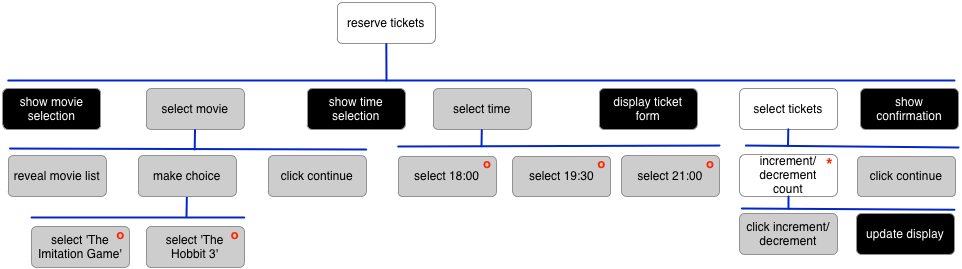
\includegraphics[scale=0.55,angle=45]{media/jsd.png}


\end{document}
